\documentclass[1p]{elsarticle_modified}
%\bibliographystyle{elsarticle-num}

%\usepackage[colorlinks]{hyperref}
%\usepackage{abbrmath_seonhwa} %\Abb, \Ascr, \Acal ,\Abf, \Afrak
\usepackage{amsfonts}
\usepackage{amssymb}
\usepackage{amsmath}
\usepackage{amsthm}
\usepackage{scalefnt}
\usepackage{amsbsy}
\usepackage{kotex}
\usepackage{caption}
\usepackage{subfig}
\usepackage{color}
\usepackage{graphicx}
\usepackage{xcolor} %% white, black, red, green, blue, cyan, magenta, yellow
\usepackage{float}
\usepackage{setspace}
\usepackage{hyperref}

\usepackage{tikz}
\usetikzlibrary{arrows}

\usepackage{multirow}
\usepackage{array} % fixed length table
\usepackage{hhline}

%%%%%%%%%%%%%%%%%%%%%
\makeatletter
\renewcommand*\env@matrix[1][\arraystretch]{%
	\edef\arraystretch{#1}%
	\hskip -\arraycolsep
	\let\@ifnextchar\new@ifnextchar
	\array{*\c@MaxMatrixCols c}}
\makeatother %https://tex.stackexchange.com/questions/14071/how-can-i-increase-the-line-spacing-in-a-matrix
%%%%%%%%%%%%%%%

\usepackage[normalem]{ulem}

\newcommand{\msout}[1]{\ifmmode\text{\sout{\ensuremath{#1}}}\else\sout{#1}\fi}
%SOURCE: \msout is \stkout macro in https://tex.stackexchange.com/questions/20609/strikeout-in-math-mode

\newcommand{\cancel}[1]{
	\ifmmode
	{\color{red}\msout{#1}}
	\else
	{\color{red}\sout{#1}}
	\fi
}

\newcommand{\add}[1]{
	{\color{blue}\uwave{#1}}
}

\newcommand{\replace}[2]{
	\ifmmode
	{\color{red}\msout{#1}}{\color{blue}\uwave{#2}}
	\else
	{\color{red}\sout{#1}}{\color{blue}\uwave{#2}}
	\fi
}

\newcommand{\Sol}{\mathcal{S}} %segment
\newcommand{\D}{D} %diagram
\newcommand{\A}{\mathcal{A}} %arc


%%%%%%%%%%%%%%%%%%%%%%%%%%%%%5 test

\def\sl{\operatorname{\textup{SL}}(2,\Cbb)}
\def\psl{\operatorname{\textup{PSL}}(2,\Cbb)}
\def\quan{\mkern 1mu \triangleright \mkern 1mu}

\theoremstyle{definition}
\newtheorem{thm}{Theorem}[section]
\newtheorem{prop}[thm]{Proposition}
\newtheorem{lem}[thm]{Lemma}
\newtheorem{ques}[thm]{Question}
\newtheorem{cor}[thm]{Corollary}
\newtheorem{defn}[thm]{Definition}
\newtheorem{exam}[thm]{Example}
\newtheorem{rmk}[thm]{Remark}
\newtheorem{alg}[thm]{Algorithm}

\newcommand{\I}{\sqrt{-1}}
\begin{document}

%\begin{frontmatter}
%
%\title{Boundary parabolic representations of knots up to 8 crossings}
%
%%% Group authors per affiliation:
%\author{Yunhi Cho} 
%\address{Department of Mathematics, University of Seoul, Seoul, Korea}
%\ead{yhcho@uos.ac.kr}
%
%
%\author{Seonhwa Kim} %\fnref{s_kim}}
%\address{Center for Geometry and Physics, Institute for Basic Science, Pohang, 37673, Korea}
%\ead{ryeona17@ibs.re.kr}
%
%\author{Hyuk Kim}
%\address{Department of Mathematical Sciences, Seoul National University, Seoul 08826, Korea}
%\ead{hyukkim@snu.ac.kr}
%
%\author{Seokbeom Yoon}
%\address{Department of Mathematical Sciences, Seoul National University, Seoul, 08826,  Korea}
%\ead{sbyoon15@snu.ac.kr}
%
%\begin{abstract}
%We find all boundary parabolic representation of knots up to 8 crossings.
%
%\end{abstract}
%\begin{keyword}
%    \MSC[2010] 57M25 
%\end{keyword}
%
%\end{frontmatter}

%\linenumbers
%\tableofcontents
%
\newcommand\colored[1]{\textcolor{white}{\rule[-0.35ex]{0.8em}{1.4ex}}\kern-0.8em\color{red} #1}%
%\newcommand\colored[1]{\textcolor{white}{ #1}\kern-2.17ex	\textcolor{white}{ #1}\kern-1.81ex	\textcolor{white}{ #1}\kern-2.15ex\color{red}#1	}

{\Large $\underline{12n_{0690}~(K12n_{0690})}$}

\setlength{\tabcolsep}{10pt}
\renewcommand{\arraystretch}{1.6}
\vspace{1cm}\begin{tabular}{m{100pt}>{\centering\arraybackslash}m{274pt}}
\multirow{5}{120pt}{
	\centering
	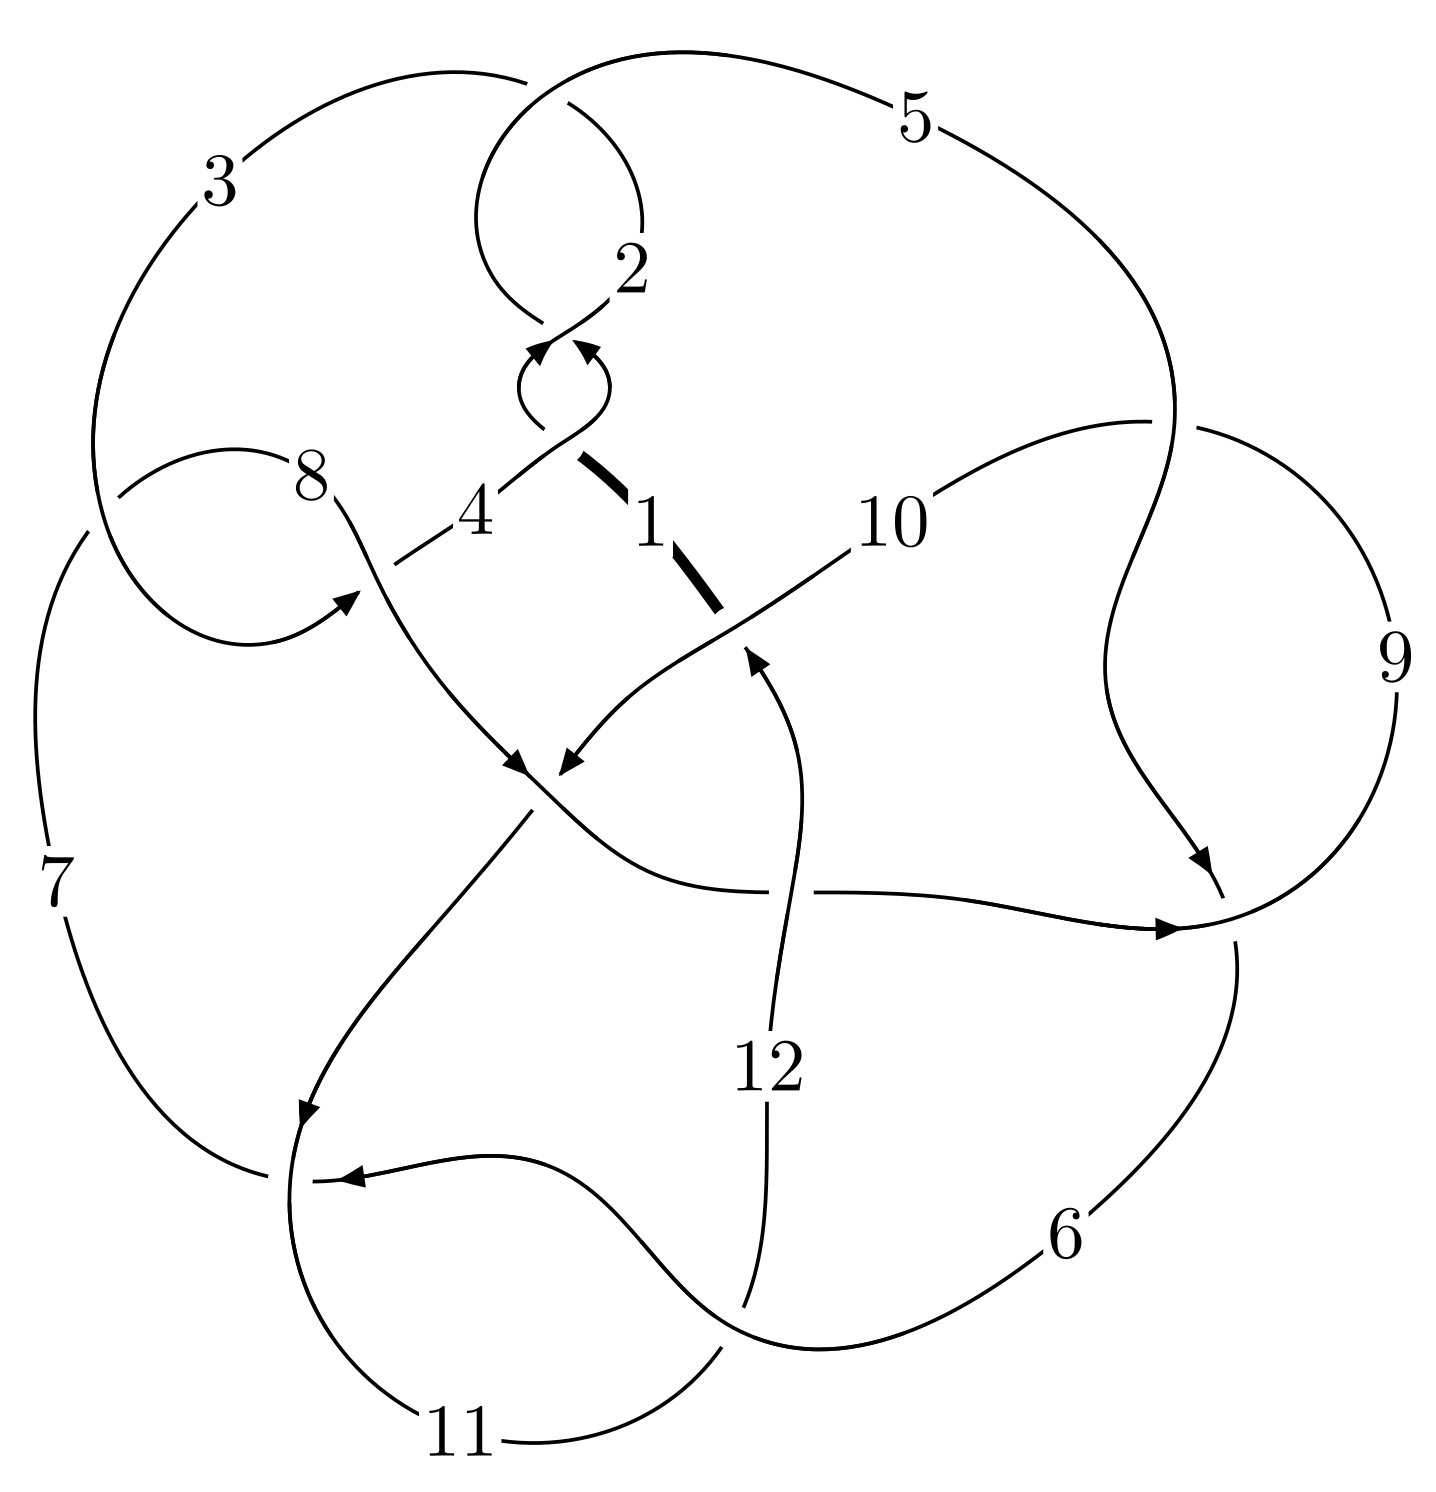
\includegraphics[width=112pt]{../../../GIT/diagram.site/Diagrams/png/2779_12n_0690.png}\\
\ \ \ A knot diagram\footnotemark}&
\allowdisplaybreaks
\textbf{Linearized knot diagam} \\
\cline{2-2}
 &
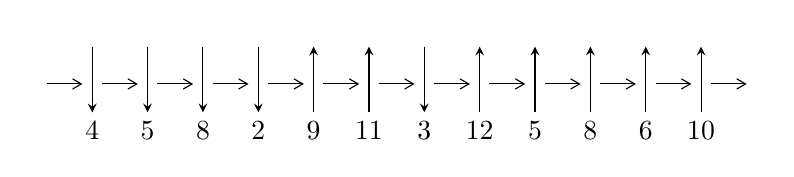
\begin{tikzpicture}[x=20pt, y=17pt]
	% nodes
	\node (C0) at (0, 0) {};
	\node (C1) at (1, 0) {};
	\node (C1U) at (1, +1) {};
	\node (C1D) at (1, -1) {4};

	\node (C2) at (2, 0) {};
	\node (C2U) at (2, +1) {};
	\node (C2D) at (2, -1) {5};

	\node (C3) at (3, 0) {};
	\node (C3U) at (3, +1) {};
	\node (C3D) at (3, -1) {8};

	\node (C4) at (4, 0) {};
	\node (C4U) at (4, +1) {};
	\node (C4D) at (4, -1) {2};

	\node (C5) at (5, 0) {};
	\node (C5U) at (5, +1) {};
	\node (C5D) at (5, -1) {9};

	\node (C6) at (6, 0) {};
	\node (C6U) at (6, +1) {};
	\node (C6D) at (6, -1) {11};

	\node (C7) at (7, 0) {};
	\node (C7U) at (7, +1) {};
	\node (C7D) at (7, -1) {3};

	\node (C8) at (8, 0) {};
	\node (C8U) at (8, +1) {};
	\node (C8D) at (8, -1) {12};

	\node (C9) at (9, 0) {};
	\node (C9U) at (9, +1) {};
	\node (C9D) at (9, -1) {5};

	\node (C10) at (10, 0) {};
	\node (C10U) at (10, +1) {};
	\node (C10D) at (10, -1) {8};

	\node (C11) at (11, 0) {};
	\node (C11U) at (11, +1) {};
	\node (C11D) at (11, -1) {6};

	\node (C12) at (12, 0) {};
	\node (C12U) at (12, +1) {};
	\node (C12D) at (12, -1) {10};
	\node (C13) at (13, 0) {};

	% arrows
	\draw[->,>={angle 60}]
	(C0) edge (C1) (C1) edge (C2) (C2) edge (C3) (C3) edge (C4) (C4) edge (C5) (C5) edge (C6) (C6) edge (C7) (C7) edge (C8) (C8) edge (C9) (C9) edge (C10) (C10) edge (C11) (C11) edge (C12) (C12) edge (C13) ;	\draw[->,>=stealth]
	(C1U) edge (C1D) (C2U) edge (C2D) (C3U) edge (C3D) (C4U) edge (C4D) (C5D) edge (C5U) (C6D) edge (C6U) (C7U) edge (C7D) (C8D) edge (C8U) (C9D) edge (C9U) (C10D) edge (C10U) (C11D) edge (C11U) (C12D) edge (C12U) ;
	\end{tikzpicture} \\
\hhline{~~} \\& 
\textbf{Solving Sequence} \\ \cline{2-2} 
 &
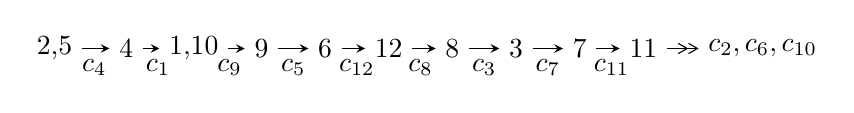
\begin{tikzpicture}[x=23pt, y=7pt]
	% node
	\node (A0) at (-1/8, 0) {2,5};
	\node (A1) at (1, 0) {4};
	\node (A2) at (33/16, 0) {1,10};
	\node (A3) at (25/8, 0) {9};
	\node (A4) at (33/8, 0) {6};
	\node (A5) at (41/8, 0) {12};
	\node (A6) at (49/8, 0) {8};
	\node (A7) at (57/8, 0) {3};
	\node (A8) at (65/8, 0) {7};
	\node (A9) at (73/8, 0) {11};
	\node (C1) at (1/2, -1) {$c_{4}$};
	\node (C2) at (3/2, -1) {$c_{1}$};
	\node (C3) at (21/8, -1) {$c_{9}$};
	\node (C4) at (29/8, -1) {$c_{5}$};
	\node (C5) at (37/8, -1) {$c_{12}$};
	\node (C6) at (45/8, -1) {$c_{8}$};
	\node (C7) at (53/8, -1) {$c_{3}$};
	\node (C8) at (61/8, -1) {$c_{7}$};
	\node (C9) at (69/8, -1) {$c_{11}$};
	\node (A10) at (11, 0) {$c_{2},c_{6},c_{10}$};

	% edge
	\draw[->,>=stealth]	
	(A0) edge (A1) (A1) edge (A2) (A2) edge (A3) (A3) edge (A4) (A4) edge (A5) (A5) edge (A6) (A6) edge (A7) (A7) edge (A8) (A8) edge (A9) ;
	\draw[->>,>={angle 60}]	
	(A9) edge (A10);
\end{tikzpicture} \\ 

\end{tabular} \\

\footnotetext{
The image of knot diagram is generated by the software ``\textbf{Draw programme}" developed by Andrew Bartholomew(\url{http://www.layer8.co.uk/maths/draw/index.htm\#Running-draw}), where we modified some parts for our purpose(\url{https://github.com/CATsTAILs/LinksPainter}).
}\phantom \\ \newline 
\centering \textbf{Ideals for irreducible components\footnotemark of $X_{\text{par}}$} 
 
\begin{align*}
I^u_{1}&=\langle 
-2.93346\times10^{17} u^{21}+1.10518\times10^{18} u^{20}+\cdots+6.77435\times10^{18} b+2.05511\times10^{18},\\
\phantom{I^u_{1}}&\phantom{= \langle  }-4.34516\times10^{16} u^{21}+5.25657\times10^{17} u^{20}+\cdots+6.77435\times10^{18} a-3.58257\times10^{19},\\
\phantom{I^u_{1}}&\phantom{= \langle  }u^{22}-5 u^{21}+\cdots+108 u+16\rangle \\
I^u_{2}&=\langle 
- u^4 a^2+5 u^4 a+\cdots+3 a-3,\;u^4 a^3+5 u^4 a^2+\cdots+27 a+31,\;u^5-2 u^4+2 u^3+u^2- u+1\rangle \\
I^u_{3}&=\langle 
2 a^2+2 b+3 a+2,\;4 a^3+4 a^2+5 a+4,\;u+1\rangle \\
I^u_{4}&=\langle 
u^{12}-3 u^{11}+u^{10}+6 u^9-6 u^8-5 u^7+7 u^6+2 u^5-2 u^4+2 u^3- u^2+b-3 u-1,\\
\phantom{I^u_{4}}&\phantom{= \langle  }- u^{12}+4 u^{11}-5 u^{10}-2 u^9+12 u^8-12 u^7+3 u^6+6 u^5-12 u^4+7 u^3+a+1,\\
\phantom{I^u_{4}}&\phantom{= \langle  }u^{13}-5 u^{12}+8 u^{11}+u^{10}-18 u^9+18 u^8+2 u^7-13 u^6+10 u^5-5 u^4-3 u^3+3 u^2+u+1\rangle \\
I^u_{5}&=\langle 
b^2+b a- a,\;a^2+a+1,\;u+1\rangle \\
\\
\end{align*}
\raggedright * 5 irreducible components of $\dim_{\mathbb{C}}=0$, with total 62 representations.\\
\footnotetext{All coefficients of polynomials are rational numbers. But the coefficients are sometimes approximated in decimal forms when there is not enough margin.}
\newpage
\renewcommand{\arraystretch}{1}
\centering \section*{I. $I^u_{1}= \langle -2.93\times10^{17} u^{21}+1.11\times10^{18} u^{20}+\cdots+6.77\times10^{18} b+2.06\times10^{18},\;-4.35\times10^{16} u^{21}+5.26\times10^{17} u^{20}+\cdots+6.77\times10^{18} a-3.58\times10^{19},\;u^{22}-5 u^{21}+\cdots+108 u+16 \rangle$}
\flushleft \textbf{(i) Arc colorings}\\
\begin{tabular}{m{7pt} m{180pt} m{7pt} m{180pt} }
\flushright $a_{2}=$&$\begin{pmatrix}0\\u\end{pmatrix}$ \\
\flushright $a_{5}=$&$\begin{pmatrix}1\\0\end{pmatrix}$ \\
\flushright $a_{4}=$&$\begin{pmatrix}1\\- u^2\end{pmatrix}$ \\
\flushright $a_{1}=$&$\begin{pmatrix}u\\- u^3+u\end{pmatrix}$ \\
\flushright $a_{10}=$&$\begin{pmatrix}0.00641415 u^{21}-0.0775953 u^{20}+\cdots+4.28301 u+5.28844\\0.0433025 u^{21}-0.163141 u^{20}+\cdots-5.64620 u-0.303366\end{pmatrix}$ \\
\flushright $a_{9}=$&$\begin{pmatrix}-0.0368883 u^{21}+0.0855460 u^{20}+\cdots+9.92921 u+5.59180\\0.0433025 u^{21}-0.163141 u^{20}+\cdots-5.64620 u-0.303366\end{pmatrix}$ \\
\flushright $a_{6}=$&$\begin{pmatrix}-0.0252335 u^{21}+0.102422 u^{20}+\cdots+0.204852 u-0.803579\\0.0147201 u^{21}-0.0585005 u^{20}+\cdots-0.406958 u-0.266094\end{pmatrix}$ \\
\flushright $a_{12}=$&$\begin{pmatrix}0.0213809 u^{21}-0.116096 u^{20}+\cdots+1.68488 u+3.12427\\-0.0129002 u^{21}+0.0465450 u^{20}+\cdots+0.617134 u+0.230969\end{pmatrix}$ \\
\flushright $a_{8}=$&$\begin{pmatrix}0.0620474 u^{21}-0.266688 u^{20}+\cdots-4.65907 u+1.63431\\-0.0435486 u^{21}+0.186762 u^{20}+\cdots+5.06681 u+0.992758\end{pmatrix}$ \\
\flushright $a_{3}=$&$\begin{pmatrix}- u\\u\end{pmatrix}$ \\
\flushright $a_{7}=$&$\begin{pmatrix}0.0771001 u^{21}-0.323949 u^{20}+\cdots-6.31235 u+1.43322\\-0.0586013 u^{21}+0.244022 u^{20}+\cdots+6.72009 u+1.19384\end{pmatrix}$ \\
\flushright $a_{11}=$&$\begin{pmatrix}0.122920 u^{21}-0.520465 u^{20}+\cdots-8.71637 u+2.14038\\-0.0963555 u^{21}+0.373312 u^{20}+\cdots+10.0845 u+1.56072\end{pmatrix}$\\&\end{tabular}
\flushleft \textbf{(ii) Obstruction class $= -1$}\\~\\
\flushleft \textbf{(iii) Cusp Shapes $= \frac{14355148220565440769}{27097382097032209472} u^{21}-\frac{32455260689474630771}{13548691048516104736} u^{20}+\cdots-\frac{224275806594788262169}{6774345524258052368} u+\frac{14951472397892805561}{1693586381064513092}$}\\~\\
\newpage\renewcommand{\arraystretch}{1}
\flushleft \textbf{(iv) u-Polynomials at the component}\newline \\
\begin{tabular}{m{50pt}|m{274pt}}
Crossings & \hspace{64pt}u-Polynomials at each crossing \\
\hline $$\begin{aligned}c_{1},c_{2},c_{4}\end{aligned}$$&$\begin{aligned}
&u^{22}-5 u^{21}+\cdots+108 u+16
\end{aligned}$\\
\hline $$\begin{aligned}c_{3},c_{7}\end{aligned}$$&$\begin{aligned}
&u^{22}-6 u^{21}+\cdots+160 u-128
\end{aligned}$\\
\hline $$\begin{aligned}c_{5},c_{6},c_{9}\\c_{11}\end{aligned}$$&$\begin{aligned}
&u^{22}+6 u^{20}+\cdots- u-1
\end{aligned}$\\
\hline $$\begin{aligned}c_{8}\end{aligned}$$&$\begin{aligned}
&u^{22}-14 u^{21}+\cdots-464 u+32
\end{aligned}$\\
\hline $$\begin{aligned}c_{10},c_{12}\end{aligned}$$&$\begin{aligned}
&u^{22}+3 u^{21}+\cdots+u+1
\end{aligned}$\\
\hline
\end{tabular}\\~\\
\newpage\renewcommand{\arraystretch}{1}
\flushleft \textbf{(v) Riley Polynomials at the component}\newline \\
\begin{tabular}{m{50pt}|m{274pt}}
Crossings & \hspace{64pt}Riley Polynomials at each crossing \\
\hline $$\begin{aligned}c_{1},c_{2},c_{4}\end{aligned}$$&$\begin{aligned}
&y^{22}-11 y^{21}+\cdots-10352 y+256
\end{aligned}$\\
\hline $$\begin{aligned}c_{3},c_{7}\end{aligned}$$&$\begin{aligned}
&y^{22}+12 y^{21}+\cdots-289792 y+16384
\end{aligned}$\\
\hline $$\begin{aligned}c_{5},c_{6},c_{9}\\c_{11}\end{aligned}$$&$\begin{aligned}
&y^{22}+12 y^{21}+\cdots-15 y+1
\end{aligned}$\\
\hline $$\begin{aligned}c_{8}\end{aligned}$$&$\begin{aligned}
&y^{22}+6 y^{21}+\cdots-36608 y+1024
\end{aligned}$\\
\hline $$\begin{aligned}c_{10},c_{12}\end{aligned}$$&$\begin{aligned}
&y^{22}-37 y^{21}+\cdots-141 y+1
\end{aligned}$\\
\hline
\end{tabular}\\~\\
\newpage\flushleft \textbf{(vi) Complex Volumes and Cusp Shapes}
$$\begin{array}{c|c|c}  
\text{Solutions to }I^u_{1}& \I (\text{vol} + \sqrt{-1}CS) & \text{Cusp shape}\\
 \hline 
\begin{aligned}
u &= -0.593822 + 0.658603 I \\
a &= -0.232154 + 0.275565 I \\
b &= -0.443126 + 0.548064 I\end{aligned}
 & -1.76571 + 0.41277 I & -1.52576 - 0.47761 I \\ \hline\begin{aligned}
u &= -0.593822 - 0.658603 I \\
a &= -0.232154 - 0.275565 I \\
b &= -0.443126 - 0.548064 I\end{aligned}
 & -1.76571 - 0.41277 I & -1.52576 + 0.47761 I \\ \hline\begin{aligned}
u &= -0.871168\phantom{ +0.000000I} \\
a &= -0.718681\phantom{ +0.000000I} \\
b &= -0.283731\phantom{ +0.000000I}\end{aligned}
 & -1.22854\phantom{ +0.000000I} & -10.9960\phantom{ +0.000000I} \\ \hline\begin{aligned}
u &= \phantom{-}1.143630 + 0.105102 I \\
a &= -0.057070 - 0.907033 I \\
b &= -0.19308 + 1.40671 I\end{aligned}
 & -11.40350 - 5.37019 I & -14.2310 + 9.8207 I \\ \hline\begin{aligned}
u &= \phantom{-}1.143630 - 0.105102 I \\
a &= -0.057070 + 0.907033 I \\
b &= -0.19308 - 1.40671 I\end{aligned}
 & -11.40350 + 5.37019 I & -14.2310 - 9.8207 I \\ \hline\begin{aligned}
u &= -0.551985 + 0.412677 I \\
a &= \phantom{-}2.14943 - 0.33347 I \\
b &= \phantom{-}0.514816 + 0.271439 I\end{aligned}
 & \phantom{-}0.924854 + 0.158726 I & \phantom{-}4.34440 - 6.69903 I \\ \hline\begin{aligned}
u &= -0.551985 - 0.412677 I \\
a &= \phantom{-}2.14943 + 0.33347 I \\
b &= \phantom{-}0.514816 - 0.271439 I\end{aligned}
 & \phantom{-}0.924854 - 0.158726 I & \phantom{-}4.34440 + 6.69903 I \\ \hline\begin{aligned}
u &= -0.864951 + 1.007370 I \\
a &= -1.007060 + 0.230412 I \\
b &= -0.863800 - 0.926848 I\end{aligned}
 & -1.67557 + 5.53623 I & -0.55960 - 5.41231 I \\ \hline\begin{aligned}
u &= -0.864951 - 1.007370 I \\
a &= -1.007060 - 0.230412 I \\
b &= -0.863800 + 0.926848 I\end{aligned}
 & -1.67557 - 5.53623 I & -0.55960 + 5.41231 I \\ \hline\begin{aligned}
u &= \phantom{-}0.636703 + 1.182420 I \\
a &= -0.620154 - 0.137775 I \\
b &= -0.861446 - 0.939694 I\end{aligned}
 & \phantom{-}7.30571 - 0.11649 I & \phantom{-}1.357790 - 0.220682 I\\
 \hline 
 \end{array}$$\newpage$$\begin{array}{c|c|c}  
\text{Solutions to }I^u_{1}& \I (\text{vol} + \sqrt{-1}CS) & \text{Cusp shape}\\
 \hline 
\begin{aligned}
u &= \phantom{-}0.636703 - 1.182420 I \\
a &= -0.620154 + 0.137775 I \\
b &= -0.861446 + 0.939694 I\end{aligned}
 & \phantom{-}7.30571 + 0.11649 I & \phantom{-}1.357790 + 0.220682 I \\ \hline\begin{aligned}
u &= \phantom{-}1.46880 + 0.23288 I \\
a &= \phantom{-}0.344293 + 0.498724 I \\
b &= -0.233614 - 0.763468 I\end{aligned}
 & -8.21433 - 3.59803 I & -0.94605 + 7.25200 I \\ \hline\begin{aligned}
u &= \phantom{-}1.46880 - 0.23288 I \\
a &= \phantom{-}0.344293 - 0.498724 I \\
b &= -0.233614 + 0.763468 I\end{aligned}
 & -8.21433 + 3.59803 I & -0.94605 - 7.25200 I \\ \hline\begin{aligned}
u &= \phantom{-}1.29164 + 0.77827 I \\
a &= -1.062860 - 0.754268 I \\
b &= -0.540251 + 1.195250 I\end{aligned}
 & \phantom{-}5.05931 - 7.06255 I & -1.67212 + 4.37965 I \\ \hline\begin{aligned}
u &= \phantom{-}1.29164 - 0.77827 I \\
a &= -1.062860 + 0.754268 I \\
b &= -0.540251 - 1.195250 I\end{aligned}
 & \phantom{-}5.05931 + 7.06255 I & -1.67212 - 4.37965 I \\ \hline\begin{aligned}
u &= -1.51290 + 0.00522 I \\
a &= -0.178858 + 0.739842 I \\
b &= \phantom{-}0.667548 - 0.729025 I\end{aligned}
 & -3.75642 - 2.26076 I & -0.68469 + 3.46770 I \\ \hline\begin{aligned}
u &= -1.51290 - 0.00522 I \\
a &= -0.178858 - 0.739842 I \\
b &= \phantom{-}0.667548 + 0.729025 I\end{aligned}
 & -3.75642 + 2.26076 I & -0.68469 - 3.46770 I \\ \hline\begin{aligned}
u &= \phantom{-}0.65142 + 1.38092 I \\
a &= \phantom{-}0.480434 + 0.328699 I \\
b &= \phantom{-}1.05295 + 1.31649 I\end{aligned}
 & \phantom{-}5.55369 + 6.92717 I & \phantom{-}0.41712 - 3.63279 I \\ \hline\begin{aligned}
u &= \phantom{-}0.65142 - 1.38092 I \\
a &= \phantom{-}0.480434 - 0.328699 I \\
b &= \phantom{-}1.05295 - 1.31649 I\end{aligned}
 & \phantom{-}5.55369 - 6.92717 I & \phantom{-}0.41712 + 3.63279 I \\ \hline\begin{aligned}
u &= \phantom{-}1.35088 + 0.88382 I \\
a &= \phantom{-}1.167610 + 0.664320 I \\
b &= \phantom{-}0.82472 - 1.52688 I\end{aligned}
 & \phantom{-}3.1876 - 14.9988 I & -1.61073 + 7.00884 I\\
 \hline 
 \end{array}$$\newpage$$\begin{array}{c|c|c}  
\text{Solutions to }I^u_{1}& \I (\text{vol} + \sqrt{-1}CS) & \text{Cusp shape}\\
 \hline 
\begin{aligned}
u &= \phantom{-}1.35088 - 0.88382 I \\
a &= \phantom{-}1.167610 - 0.664320 I \\
b &= \phantom{-}0.82472 + 1.52688 I\end{aligned}
 & \phantom{-}3.1876 + 14.9988 I & -1.61073 - 7.00884 I \\ \hline\begin{aligned}
u &= -0.167658\phantom{ +0.000000I} \\
a &= \phantom{-}4.50144\phantom{ +0.000000I} \\
b &= \phantom{-}0.434292\phantom{ +0.000000I}\end{aligned}
 & \phantom{-}0.927721\phantom{ +0.000000I} & \phantom{-}12.4670\phantom{ +0.000000I}\\
 \hline 
 \end{array}$$\newpage\newpage\renewcommand{\arraystretch}{1}
\centering \section*{II. $I^u_{2}= \langle - u^4 a^2+5 u^4 a+\cdots+3 a-3,\;u^4 a^3+5 u^4 a^2+\cdots+27 a+31,\;u^5-2 u^4+2 u^3+u^2- u+1 \rangle$}
\flushleft \textbf{(i) Arc colorings}\\
\begin{tabular}{m{7pt} m{180pt} m{7pt} m{180pt} }
\flushright $a_{2}=$&$\begin{pmatrix}0\\u\end{pmatrix}$ \\
\flushright $a_{5}=$&$\begin{pmatrix}1\\0\end{pmatrix}$ \\
\flushright $a_{4}=$&$\begin{pmatrix}1\\- u^2\end{pmatrix}$ \\
\flushright $a_{1}=$&$\begin{pmatrix}u\\- u^3+u\end{pmatrix}$ \\
\flushright $a_{10}=$&$\begin{pmatrix}a\\\frac{1}{2} u^4 a^2-\frac{5}{2} u^4 a+\cdots-\frac{3}{2} a+\frac{3}{2}\end{pmatrix}$ \\
\flushright $a_{9}=$&$\begin{pmatrix}-\frac{1}{2} u^4 a^2+\frac{5}{2} u^4 a+\cdots+\frac{5}{2} a-\frac{3}{2}\\\frac{1}{2} u^4 a^2-\frac{5}{2} u^4 a+\cdots-\frac{3}{2} a+\frac{3}{2}\end{pmatrix}$ \\
\flushright $a_{6}=$&$\begin{pmatrix}2 u^4 a^3-3 u^4 a^2+\cdots- a^2-6\\-\frac{5}{2} u^4 a^3+\frac{7}{2} u^4 a^2+\cdots-\frac{9}{2} a+5\end{pmatrix}$ \\
\flushright $a_{12}=$&$\begin{pmatrix}-\frac{1}{2} u^4 a^3+\frac{1}{2} u^4 a^2+\cdots-\frac{7}{2} a-7\\\frac{3}{2} u^4 a^3-\frac{5}{2} u^4 a^2+\cdots+\frac{5}{2} a-5\end{pmatrix}$ \\
\flushright $a_{8}=$&$\begin{pmatrix}- u^4+2 u^3- u^2-2 u+1\\- u^3+u^2-1\end{pmatrix}$ \\
\flushright $a_{3}=$&$\begin{pmatrix}- u\\u\end{pmatrix}$ \\
\flushright $a_{7}=$&$\begin{pmatrix}- u^4+3 u^3- u^2-2 u+2\\-2 u^3+u^2-2\end{pmatrix}$ \\
\flushright $a_{11}=$&$\begin{pmatrix}-\frac{3}{2} u^4 a^2+\frac{3}{2} u^4 a+\cdots+\frac{1}{2} a-\frac{21}{2}\\u^4 a^3- u^4 a^2+\cdots-4 a^2+3\end{pmatrix}$\\&\end{tabular}
\flushleft \textbf{(ii) Obstruction class $= -1$}\\~\\
\flushleft \textbf{(iii) Cusp Shapes $= 4 u^4 a^2-4 a^3 u-4 a^2 u^2+4 u^3 a-16 u^4-4 a^3+12 a^2 u-8 u^2 a+26 u^3+8 a^2+16 a u-28 u^2-4 a-2 u-24$}\\~\\
\newpage\renewcommand{\arraystretch}{1}
\flushleft \textbf{(iv) u-Polynomials at the component}\newline \\
\begin{tabular}{m{50pt}|m{274pt}}
Crossings & \hspace{64pt}u-Polynomials at each crossing \\
\hline $$\begin{aligned}c_{1},c_{2},c_{4}\end{aligned}$$&$\begin{aligned}
&(u^5-2 u^4+2 u^3+u^2- u+1)^4
\end{aligned}$\\
\hline $$\begin{aligned}c_{3},c_{7}\end{aligned}$$&$\begin{aligned}
&(u^5+u^4+5 u^3+u^2+2 u-2)^4
\end{aligned}$\\
\hline $$\begin{aligned}c_{5},c_{6},c_{9}\\c_{11}\end{aligned}$$&$\begin{aligned}
&u^{20}-2 u^{19}+\cdots+150 u+103
\end{aligned}$\\
\hline $$\begin{aligned}c_{8}\end{aligned}$$&$\begin{aligned}
&(u^2+u+1)^{10}
\end{aligned}$\\
\hline $$\begin{aligned}c_{10},c_{12}\end{aligned}$$&$\begin{aligned}
&u^{20}+2 u^{19}+\cdots+13224 u+2521
\end{aligned}$\\
\hline
\end{tabular}\\~\\
\newpage\renewcommand{\arraystretch}{1}
\flushleft \textbf{(v) Riley Polynomials at the component}\newline \\
\begin{tabular}{m{50pt}|m{274pt}}
Crossings & \hspace{64pt}Riley Polynomials at each crossing \\
\hline $$\begin{aligned}c_{1},c_{2},c_{4}\end{aligned}$$&$\begin{aligned}
&(y^5+6 y^3- y^2- y-1)^4
\end{aligned}$\\
\hline $$\begin{aligned}c_{3},c_{7}\end{aligned}$$&$\begin{aligned}
&(y^5+9 y^4+27 y^3+23 y^2+8 y-4)^4
\end{aligned}$\\
\hline $$\begin{aligned}c_{5},c_{6},c_{9}\\c_{11}\end{aligned}$$&$\begin{aligned}
&y^{20}+6 y^{19}+\cdots+110988 y+10609
\end{aligned}$\\
\hline $$\begin{aligned}c_{8}\end{aligned}$$&$\begin{aligned}
&(y^2+y+1)^{10}
\end{aligned}$\\
\hline $$\begin{aligned}c_{10},c_{12}\end{aligned}$$&$\begin{aligned}
&y^{20}-18 y^{19}+\cdots+37696544 y+6355441
\end{aligned}$\\
\hline
\end{tabular}\\~\\
\newpage\flushleft \textbf{(vi) Complex Volumes and Cusp Shapes}
$$\begin{array}{c|c|c}  
\text{Solutions to }I^u_{2}& \I (\text{vol} + \sqrt{-1}CS) & \text{Cusp shape}\\
 \hline 
\begin{aligned}
u &= -0.833800\phantom{ +0.000000I} \\
a &= -2.41812 + 0.15016 I \\
b &= -0.272476 - 1.364140 I\end{aligned}
 & -6.13845 + 2.02988 I & -10.94304 - 3.46410 I \\ \hline\begin{aligned}
u &= -0.833800\phantom{ +0.000000I} \\
a &= -2.41812 - 0.15016 I \\
b &= -0.272476 + 1.364140 I\end{aligned}
 & -6.13845 - 2.02988 I & -10.94304 + 3.46410 I \\ \hline\begin{aligned}
u &= -0.833800\phantom{ +0.000000I} \\
a &= -0.91730 + 5.62696 I \\
b &= \phantom{-}0.409925 + 1.126070 I\end{aligned}
 & -6.13845 + 2.02988 I & -10.94304 - 3.46410 I \\ \hline\begin{aligned}
u &= -0.833800\phantom{ +0.000000I} \\
a &= -0.91730 - 5.62696 I \\
b &= \phantom{-}0.409925 - 1.126070 I\end{aligned}
 & -6.13845 - 2.02988 I & -10.94304 + 3.46410 I \\ \hline\begin{aligned}
u &= \phantom{-}0.317129 + 0.618084 I \\
a &= -1.226670 - 0.088438 I \\
b &= -0.05655 + 1.55273 I\end{aligned}
 & -3.08342 + 0.92097 I & \phantom{-}0.36548 - 1.42298 I \\ \hline\begin{aligned}
u &= \phantom{-}0.317129 + 0.618084 I \\
a &= -1.283840 - 0.195995 I \\
b &= -1.102440 + 0.773065 I\end{aligned}
 & -3.08342 - 3.13880 I & \phantom{-}0.36548 + 5.50523 I \\ \hline\begin{aligned}
u &= \phantom{-}0.317129 + 0.618084 I \\
a &= \phantom{-}1.42128 - 0.76900 I \\
b &= -0.035904 - 0.509258 I\end{aligned}
 & -3.08342 + 0.92097 I & \phantom{-}0.36548 - 1.42298 I \\ \hline\begin{aligned}
u &= \phantom{-}0.317129 + 0.618084 I \\
a &= \phantom{-}1.92910 + 0.79325 I \\
b &= \phantom{-}0.244995 - 1.374870 I\end{aligned}
 & -3.08342 - 3.13880 I & \phantom{-}0.36548 + 5.50523 I \\ \hline\begin{aligned}
u &= \phantom{-}0.317129 - 0.618084 I \\
a &= -1.226670 + 0.088438 I \\
b &= -0.05655 - 1.55273 I\end{aligned}
 & -3.08342 - 0.92097 I & \phantom{-}0.36548 + 1.42298 I \\ \hline\begin{aligned}
u &= \phantom{-}0.317129 - 0.618084 I \\
a &= -1.283840 + 0.195995 I \\
b &= -1.102440 - 0.773065 I\end{aligned}
 & -3.08342 + 3.13880 I & \phantom{-}0.36548 - 5.50523 I\\
 \hline 
 \end{array}$$\newpage$$\begin{array}{c|c|c}  
\text{Solutions to }I^u_{2}& \I (\text{vol} + \sqrt{-1}CS) & \text{Cusp shape}\\
 \hline 
\begin{aligned}
u &= \phantom{-}0.317129 - 0.618084 I \\
a &= \phantom{-}1.42128 + 0.76900 I \\
b &= -0.035904 + 0.509258 I\end{aligned}
 & -3.08342 - 0.92097 I & \phantom{-}0.36548 + 1.42298 I \\ \hline\begin{aligned}
u &= \phantom{-}0.317129 - 0.618084 I \\
a &= \phantom{-}1.92910 - 0.79325 I \\
b &= \phantom{-}0.244995 + 1.374870 I\end{aligned}
 & -3.08342 + 3.13880 I & \phantom{-}0.36548 - 5.50523 I \\ \hline\begin{aligned}
u &= \phantom{-}1.09977 + 1.12945 I \\
a &= \phantom{-}0.969002 + 0.567215 I \\
b &= \phantom{-}1.49281 - 1.00208 I\end{aligned}
 & \phantom{-}6.97511 - 2.09502 I & -0.89396 - 1.30967 I \\ \hline\begin{aligned}
u &= \phantom{-}1.09977 + 1.12945 I \\
a &= -1.097140 - 0.256413 I \\
b &= -0.722774 + 1.025520 I\end{aligned}
 & \phantom{-}6.97511 - 6.15479 I & -0.89396 + 5.61853 I \\ \hline\begin{aligned}
u &= \phantom{-}1.09977 + 1.12945 I \\
a &= \phantom{-}0.555611 + 0.563935 I \\
b &= \phantom{-}1.77894 + 0.45753 I\end{aligned}
 & \phantom{-}6.97511 - 6.15479 I & -0.89396 + 5.61853 I \\ \hline\begin{aligned}
u &= \phantom{-}1.09977 + 1.12945 I \\
a &= -0.431917 - 0.251999 I \\
b &= -0.736535 - 0.654115 I\end{aligned}
 & \phantom{-}6.97511 - 2.09502 I & -0.89396 - 1.30967 I \\ \hline\begin{aligned}
u &= \phantom{-}1.09977 - 1.12945 I \\
a &= \phantom{-}0.969002 - 0.567215 I \\
b &= \phantom{-}1.49281 + 1.00208 I\end{aligned}
 & \phantom{-}6.97511 + 2.09502 I & -0.89396 + 1.30967 I \\ \hline\begin{aligned}
u &= \phantom{-}1.09977 - 1.12945 I \\
a &= -1.097140 + 0.256413 I \\
b &= -0.722774 - 1.025520 I\end{aligned}
 & \phantom{-}6.97511 + 6.15479 I & -0.89396 - 5.61853 I \\ \hline\begin{aligned}
u &= \phantom{-}1.09977 - 1.12945 I \\
a &= \phantom{-}0.555611 - 0.563935 I \\
b &= \phantom{-}1.77894 - 0.45753 I\end{aligned}
 & \phantom{-}6.97511 + 6.15479 I & -0.89396 - 5.61853 I \\ \hline\begin{aligned}
u &= \phantom{-}1.09977 - 1.12945 I \\
a &= -0.431917 + 0.251999 I \\
b &= -0.736535 + 0.654115 I\end{aligned}
 & \phantom{-}6.97511 + 2.09502 I & -0.89396 + 1.30967 I\\
 \hline 
 \end{array}$$\newpage\newpage\renewcommand{\arraystretch}{1}
\centering \section*{III. $I^u_{3}= \langle 2 a^2+2 b+3 a+2,\;4 a^3+4 a^2+5 a+4,\;u+1 \rangle$}
\flushleft \textbf{(i) Arc colorings}\\
\begin{tabular}{m{7pt} m{180pt} m{7pt} m{180pt} }
\flushright $a_{2}=$&$\begin{pmatrix}0\\-1\end{pmatrix}$ \\
\flushright $a_{5}=$&$\begin{pmatrix}1\\0\end{pmatrix}$ \\
\flushright $a_{4}=$&$\begin{pmatrix}1\\-1\end{pmatrix}$ \\
\flushright $a_{1}=$&$\begin{pmatrix}-1\\0\end{pmatrix}$ \\
\flushright $a_{10}=$&$\begin{pmatrix}a\\- a^2-\frac{3}{2} a-1\end{pmatrix}$ \\
\flushright $a_{9}=$&$\begin{pmatrix}a^2+\frac{5}{2} a+1\\- a^2-\frac{3}{2} a-1\end{pmatrix}$ \\
\flushright $a_{6}=$&$\begin{pmatrix}\frac{3}{2} a^2-\frac{3}{4} a-1\\- a^2+\frac{1}{2} a+1\end{pmatrix}$ \\
\flushright $a_{12}=$&$\begin{pmatrix}\frac{1}{2} a^2-\frac{1}{4} a-2\\- a^2+\frac{1}{2} a+1\end{pmatrix}$ \\
\flushright $a_{8}=$&$\begin{pmatrix}-2 a^2- a+1\\2 a^2+a-1\end{pmatrix}$ \\
\flushright $a_{3}=$&$\begin{pmatrix}1\\-1\end{pmatrix}$ \\
\flushright $a_{7}=$&$\begin{pmatrix}-2 a^2- a+1\\2 a^2+a-1\end{pmatrix}$ \\
\flushright $a_{11}=$&$\begin{pmatrix}-2 a^2-4 a-3\\a^2+\frac{7}{2} a+2\end{pmatrix}$\\&\end{tabular}
\flushleft \textbf{(ii) Obstruction class $= 1$}\\~\\
\flushleft \textbf{(iii) Cusp Shapes $= \frac{19}{4} a^2-\frac{11}{8} a+\frac{17}{2}$}\\~\\
\newpage\renewcommand{\arraystretch}{1}
\flushleft \textbf{(iv) u-Polynomials at the component}\newline \\
\begin{tabular}{m{50pt}|m{274pt}}
Crossings & \hspace{64pt}u-Polynomials at each crossing \\
\hline $$\begin{aligned}c_{1},c_{2}\end{aligned}$$&$\begin{aligned}
&(u-1)^3
\end{aligned}$\\
\hline $$\begin{aligned}c_{3},c_{7}\end{aligned}$$&$\begin{aligned}
&u^3
\end{aligned}$\\
\hline $$\begin{aligned}c_{4}\end{aligned}$$&$\begin{aligned}
&(u+1)^3
\end{aligned}$\\
\hline $$\begin{aligned}c_{5},c_{6}\end{aligned}$$&$\begin{aligned}
&u^3+2 u+1
\end{aligned}$\\
\hline $$\begin{aligned}c_{8}\end{aligned}$$&$\begin{aligned}
&u^3+3 u^2+5 u+2
\end{aligned}$\\
\hline $$\begin{aligned}c_{9},c_{10},c_{11}\\c_{12}\end{aligned}$$&$\begin{aligned}
&u^3+2 u-1
\end{aligned}$\\
\hline
\end{tabular}\\~\\
\newpage\renewcommand{\arraystretch}{1}
\flushleft \textbf{(v) Riley Polynomials at the component}\newline \\
\begin{tabular}{m{50pt}|m{274pt}}
Crossings & \hspace{64pt}Riley Polynomials at each crossing \\
\hline $$\begin{aligned}c_{1},c_{2},c_{4}\end{aligned}$$&$\begin{aligned}
&(y-1)^3
\end{aligned}$\\
\hline $$\begin{aligned}c_{3},c_{7}\end{aligned}$$&$\begin{aligned}
&y^3
\end{aligned}$\\
\hline $$\begin{aligned}c_{5},c_{6},c_{9}\\c_{10},c_{11},c_{12}\end{aligned}$$&$\begin{aligned}
&y^3+4 y^2+4 y-1
\end{aligned}$\\
\hline $$\begin{aligned}c_{8}\end{aligned}$$&$\begin{aligned}
&y^3+y^2+13 y-4
\end{aligned}$\\
\hline
\end{tabular}\\~\\
\newpage\flushleft \textbf{(vi) Complex Volumes and Cusp Shapes}
$$\begin{array}{c|c|c}  
\text{Solutions to }I^u_{3}& \I (\text{vol} + \sqrt{-1}CS) & \text{Cusp shape}\\
 \hline 
\begin{aligned}
u &= -1.00000\phantom{ +0.000000I} \\
a &= -0.061957 + 1.066580 I \\
b &= \phantom{-}0.22670 - 1.46771 I\end{aligned}
 & -11.08570 - 5.13794 I & \phantom{-}3.19982 - 2.09434 I \\ \hline\begin{aligned}
u &= -1.00000\phantom{ +0.000000I} \\
a &= -0.061957 - 1.066580 I \\
b &= \phantom{-}0.22670 + 1.46771 I\end{aligned}
 & -11.08570 + 5.13794 I & \phantom{-}3.19982 + 2.09434 I \\ \hline\begin{aligned}
u &= -1.00000\phantom{ +0.000000I} \\
a &= -0.876086\phantom{ +0.000000I} \\
b &= -0.453398\phantom{ +0.000000I}\end{aligned}
 & -0.857735\phantom{ +0.000000I} & \phantom{-}13.3500\phantom{ +0.000000I}\\
 \hline 
 \end{array}$$\newpage\newpage\renewcommand{\arraystretch}{1}
\centering \section*{IV. $I^u_{4}= \langle u^{12}-3 u^{11}+\cdots+b-1,\;- u^{12}+4 u^{11}+\cdots+a+1,\;u^{13}-5 u^{12}+\cdots+u+1 \rangle$}
\flushleft \textbf{(i) Arc colorings}\\
\begin{tabular}{m{7pt} m{180pt} m{7pt} m{180pt} }
\flushright $a_{2}=$&$\begin{pmatrix}0\\u\end{pmatrix}$ \\
\flushright $a_{5}=$&$\begin{pmatrix}1\\0\end{pmatrix}$ \\
\flushright $a_{4}=$&$\begin{pmatrix}1\\- u^2\end{pmatrix}$ \\
\flushright $a_{1}=$&$\begin{pmatrix}u\\- u^3+u\end{pmatrix}$ \\
\flushright $a_{10}=$&$\begin{pmatrix}u^{12}-4 u^{11}+5 u^{10}+2 u^9-12 u^8+12 u^7-3 u^6-6 u^5+12 u^4-7 u^3-1\\- u^{12}+3 u^{11}+\cdots+3 u+1\end{pmatrix}$ \\
\flushright $a_{9}=$&$\begin{pmatrix}2 u^{12}-7 u^{11}+\cdots-3 u-2\\- u^{12}+3 u^{11}+\cdots+3 u+1\end{pmatrix}$ \\
\flushright $a_{6}=$&$\begin{pmatrix}u^{12}-6 u^{11}+\cdots+3 u+1\\u^{11}-4 u^{10}+5 u^9+2 u^8-11 u^7+8 u^6+2 u^5-5 u^4+4 u^3- u^2- u+1\end{pmatrix}$ \\
\flushright $a_{12}=$&$\begin{pmatrix}- u^{11}+5 u^{10}-9 u^9+4 u^8+9 u^7-14 u^6+7 u^5- u^4-3 u^3+5 u^2- u+1\\- u^3+u^2-1\end{pmatrix}$ \\
\flushright $a_{8}=$&$\begin{pmatrix}-2 u^{12}+8 u^{11}+\cdots+u+1\\2 u^{12}-8 u^{11}+\cdots-3 u-2\end{pmatrix}$ \\
\flushright $a_{3}=$&$\begin{pmatrix}- u\\u\end{pmatrix}$ \\
\flushright $a_{7}=$&$\begin{pmatrix}-2 u^{12}+7 u^{11}+\cdots+u+1\\2 u^{12}-7 u^{11}+\cdots-3 u-2\end{pmatrix}$ \\
\flushright $a_{11}=$&$\begin{pmatrix}u^{12}-4 u^{11}+\cdots+u^2-2\\- u^{12}+3 u^{11}+\cdots+4 u+1\end{pmatrix}$\\&\end{tabular}
\flushleft \textbf{(ii) Obstruction class $= 1$}\\~\\
\flushleft \textbf{(iii) Cusp Shapes $= 11 u^{11}-46 u^{10}+62 u^9+11 u^8-114 u^7+98 u^6-4 u^5-36 u^4+51 u^3-26 u^2-10 u-9$}\\~\\
\newpage\renewcommand{\arraystretch}{1}
\flushleft \textbf{(iv) u-Polynomials at the component}\newline \\
\begin{tabular}{m{50pt}|m{274pt}}
Crossings & \hspace{64pt}u-Polynomials at each crossing \\
\hline $$\begin{aligned}c_{1},c_{2}\end{aligned}$$&$\begin{aligned}
&u^{13}+5 u^{12}+\cdots+u-1
\end{aligned}$\\
\hline $$\begin{aligned}c_{3}\end{aligned}$$&$\begin{aligned}
&u^{13}- u^{12}+\cdots- u-1
\end{aligned}$\\
\hline $$\begin{aligned}c_{4}\end{aligned}$$&$\begin{aligned}
&u^{13}-5 u^{12}+\cdots+u+1
\end{aligned}$\\
\hline $$\begin{aligned}c_{5},c_{11}\end{aligned}$$&$\begin{aligned}
&u^{13}+5 u^{11}+\cdots+8 u-1
\end{aligned}$\\
\hline $$\begin{aligned}c_{6},c_{9}\end{aligned}$$&$\begin{aligned}
&u^{13}+5 u^{11}+\cdots+8 u+1
\end{aligned}$\\
\hline $$\begin{aligned}c_{7}\end{aligned}$$&$\begin{aligned}
&u^{13}+u^{12}+\cdots- u+1
\end{aligned}$\\
\hline $$\begin{aligned}c_{8}\end{aligned}$$&$\begin{aligned}
&u^{13}-2 u^{12}+\cdots+3 u+1
\end{aligned}$\\
\hline $$\begin{aligned}c_{10},c_{12}\end{aligned}$$&$\begin{aligned}
&u^{13}-3 u^{12}+\cdots-2 u-1
\end{aligned}$\\
\hline
\end{tabular}\\~\\
\newpage\renewcommand{\arraystretch}{1}
\flushleft \textbf{(v) Riley Polynomials at the component}\newline \\
\begin{tabular}{m{50pt}|m{274pt}}
Crossings & \hspace{64pt}Riley Polynomials at each crossing \\
\hline $$\begin{aligned}c_{1},c_{2},c_{4}\end{aligned}$$&$\begin{aligned}
&y^{13}-9 y^{12}+\cdots-5 y-1
\end{aligned}$\\
\hline $$\begin{aligned}c_{3},c_{7}\end{aligned}$$&$\begin{aligned}
&y^{13}+3 y^{12}+\cdots- y-1
\end{aligned}$\\
\hline $$\begin{aligned}c_{5},c_{6},c_{9}\\c_{11}\end{aligned}$$&$\begin{aligned}
&y^{13}+10 y^{12}+\cdots+62 y-1
\end{aligned}$\\
\hline $$\begin{aligned}c_{8}\end{aligned}$$&$\begin{aligned}
&y^{13}+4 y^{12}+\cdots+3 y-1
\end{aligned}$\\
\hline $$\begin{aligned}c_{10},c_{12}\end{aligned}$$&$\begin{aligned}
&y^{13}-3 y^{12}+\cdots-4 y-1
\end{aligned}$\\
\hline
\end{tabular}\\~\\
\newpage\flushleft \textbf{(vi) Complex Volumes and Cusp Shapes}
$$\begin{array}{c|c|c}  
\text{Solutions to }I^u_{4}& \I (\text{vol} + \sqrt{-1}CS) & \text{Cusp shape}\\
 \hline 
\begin{aligned}
u &= -1.071790 + 0.063918 I \\
a &= \phantom{-}3.89373 + 0.86609 I \\
b &= -0.350540 + 1.237350 I\end{aligned}
 & -6.72126 - 1.88681 I & \phantom{-}0.50306 + 13.63564 I \\ \hline\begin{aligned}
u &= -1.071790 - 0.063918 I \\
a &= \phantom{-}3.89373 - 0.86609 I \\
b &= -0.350540 - 1.237350 I\end{aligned}
 & -6.72126 + 1.88681 I & \phantom{-}0.50306 - 13.63564 I \\ \hline\begin{aligned}
u &= \phantom{-}0.130382 + 0.815929 I \\
a &= \phantom{-}1.43598 - 0.50475 I \\
b &= \phantom{-}0.570608 - 1.217040 I\end{aligned}
 & -3.69895 - 1.30722 I & -2.19900 + 1.04986 I \\ \hline\begin{aligned}
u &= \phantom{-}0.130382 - 0.815929 I \\
a &= \phantom{-}1.43598 + 0.50475 I \\
b &= \phantom{-}0.570608 + 1.217040 I\end{aligned}
 & -3.69895 + 1.30722 I & -2.19900 - 1.04986 I \\ \hline\begin{aligned}
u &= -0.672448\phantom{ +0.000000I} \\
a &= \phantom{-}2.97967\phantom{ +0.000000I} \\
b &= \phantom{-}0.122783\phantom{ +0.000000I}\end{aligned}
 & \phantom{-}0.610906\phantom{ +0.000000I} & -22.4950\phantom{ +0.000000I} \\ \hline\begin{aligned}
u &= \phantom{-}1.384340 + 0.198421 I \\
a &= \phantom{-}0.111997 + 1.000200 I \\
b &= \phantom{-}0.163145 - 1.174190 I\end{aligned}
 & -9.90727 - 5.10044 I & -4.52290 + 4.82780 I \\ \hline\begin{aligned}
u &= \phantom{-}1.384340 - 0.198421 I \\
a &= \phantom{-}0.111997 - 1.000200 I \\
b &= \phantom{-}0.163145 + 1.174190 I\end{aligned}
 & -9.90727 + 5.10044 I & -4.52290 - 4.82780 I \\ \hline\begin{aligned}
u &= \phantom{-}1.44789 + 0.30492 I \\
a &= -0.265186 - 0.255350 I \\
b &= \phantom{-}0.378653 + 0.878868 I\end{aligned}
 & -8.51258 - 3.08878 I & -7.58668 - 3.50114 I \\ \hline\begin{aligned}
u &= \phantom{-}1.44789 - 0.30492 I \\
a &= -0.265186 + 0.255350 I \\
b &= \phantom{-}0.378653 - 0.878868 I\end{aligned}
 & -8.51258 + 3.08878 I & -7.58668 + 3.50114 I \\ \hline\begin{aligned}
u &= \phantom{-}1.10155 + 1.08640 I \\
a &= -0.805723 - 0.406507 I \\
b &= -1.082570 + 0.295127 I\end{aligned}
 & \phantom{-}7.14389 - 4.01026 I & -0.32249 + 2.61344 I\\
 \hline 
 \end{array}$$\newpage$$\begin{array}{c|c|c}  
\text{Solutions to }I^u_{4}& \I (\text{vol} + \sqrt{-1}CS) & \text{Cusp shape}\\
 \hline 
\begin{aligned}
u &= \phantom{-}1.10155 - 1.08640 I \\
a &= -0.805723 + 0.406507 I \\
b &= -1.082570 - 0.295127 I\end{aligned}
 & \phantom{-}7.14389 + 4.01026 I & -0.32249 - 2.61344 I \\ \hline\begin{aligned}
u &= -0.156146 + 0.399949 I \\
a &= -1.36064 + 0.71418 I \\
b &= \phantom{-}0.259312 + 1.270730 I\end{aligned}
 & -4.92823 + 2.67880 I & -0.12459 - 4.50580 I \\ \hline\begin{aligned}
u &= -0.156146 - 0.399949 I \\
a &= -1.36064 - 0.71418 I \\
b &= \phantom{-}0.259312 - 1.270730 I\end{aligned}
 & -4.92823 - 2.67880 I & -0.12459 + 4.50580 I\\
 \hline 
 \end{array}$$\newpage\newpage\renewcommand{\arraystretch}{1}
\centering \section*{V. $I^u_{5}= \langle b^2+b a- a,\;a^2+a+1,\;u+1 \rangle$}
\flushleft \textbf{(i) Arc colorings}\\
\begin{tabular}{m{7pt} m{180pt} m{7pt} m{180pt} }
\flushright $a_{2}=$&$\begin{pmatrix}0\\-1\end{pmatrix}$ \\
\flushright $a_{5}=$&$\begin{pmatrix}1\\0\end{pmatrix}$ \\
\flushright $a_{4}=$&$\begin{pmatrix}1\\-1\end{pmatrix}$ \\
\flushright $a_{1}=$&$\begin{pmatrix}-1\\0\end{pmatrix}$ \\
\flushright $a_{10}=$&$\begin{pmatrix}a\\b\end{pmatrix}$ \\
\flushright $a_{9}=$&$\begin{pmatrix}- b+a\\b\end{pmatrix}$ \\
\flushright $a_{6}=$&$\begin{pmatrix}-2 b a+a+1\\b a- a\end{pmatrix}$ \\
\flushright $a_{12}=$&$\begin{pmatrix}- b a-1\\b a- a\end{pmatrix}$ \\
\flushright $a_{8}=$&$\begin{pmatrix}-1\\1\end{pmatrix}$ \\
\flushright $a_{3}=$&$\begin{pmatrix}1\\-1\end{pmatrix}$ \\
\flushright $a_{7}=$&$\begin{pmatrix}-1\\1\end{pmatrix}$ \\
\flushright $a_{11}=$&$\begin{pmatrix}b+2 a\\- a\end{pmatrix}$\\&\end{tabular}
\flushleft \textbf{(ii) Obstruction class $= 1$}\\~\\
\flushleft \textbf{(iii) Cusp Shapes $= -4 a-4$}\\~\\
\newpage\renewcommand{\arraystretch}{1}
\flushleft \textbf{(iv) u-Polynomials at the component}\newline \\
\begin{tabular}{m{50pt}|m{274pt}}
Crossings & \hspace{64pt}u-Polynomials at each crossing \\
\hline $$\begin{aligned}c_{1},c_{2}\end{aligned}$$&$\begin{aligned}
&(u-1)^4
\end{aligned}$\\
\hline $$\begin{aligned}c_{3},c_{7}\end{aligned}$$&$\begin{aligned}
&u^4
\end{aligned}$\\
\hline $$\begin{aligned}c_{4}\end{aligned}$$&$\begin{aligned}
&(u+1)^4
\end{aligned}$\\
\hline $$\begin{aligned}c_{5},c_{6}\end{aligned}$$&$\begin{aligned}
&u^4- u^3+2 u^2-2 u+1
\end{aligned}$\\
\hline $$\begin{aligned}c_{8}\end{aligned}$$&$\begin{aligned}
&(u^2- u+1)^2
\end{aligned}$\\
\hline $$\begin{aligned}c_{9},c_{10},c_{11}\\c_{12}\end{aligned}$$&$\begin{aligned}
&u^4+u^3+2 u^2+2 u+1
\end{aligned}$\\
\hline
\end{tabular}\\~\\
\newpage\renewcommand{\arraystretch}{1}
\flushleft \textbf{(v) Riley Polynomials at the component}\newline \\
\begin{tabular}{m{50pt}|m{274pt}}
Crossings & \hspace{64pt}Riley Polynomials at each crossing \\
\hline $$\begin{aligned}c_{1},c_{2},c_{4}\end{aligned}$$&$\begin{aligned}
&(y-1)^4
\end{aligned}$\\
\hline $$\begin{aligned}c_{3},c_{7}\end{aligned}$$&$\begin{aligned}
&y^4
\end{aligned}$\\
\hline $$\begin{aligned}c_{5},c_{6},c_{9}\\c_{10},c_{11},c_{12}\end{aligned}$$&$\begin{aligned}
&y^4+3 y^3+2 y^2+1
\end{aligned}$\\
\hline $$\begin{aligned}c_{8}\end{aligned}$$&$\begin{aligned}
&(y^2+y+1)^2
\end{aligned}$\\
\hline
\end{tabular}\\~\\
\newpage\flushleft \textbf{(vi) Complex Volumes and Cusp Shapes}
$$\begin{array}{c|c|c}  
\text{Solutions to }I^u_{5}& \I (\text{vol} + \sqrt{-1}CS) & \text{Cusp shape}\\
 \hline 
\begin{aligned}
u &= -1.00000\phantom{ +0.000000I} \\
a &= -0.500000 + 0.866025 I \\
b &= \phantom{-}0.621744 + 0.440597 I\end{aligned}
 & -4.93480 + 2.02988 I & -2.00000 - 3.46410 I \\ \hline\begin{aligned}
u &= -1.00000\phantom{ +0.000000I} \\
a &= -0.500000 + 0.866025 I \\
b &= -0.121744 - 1.306620 I\end{aligned}
 & -4.93480 + 2.02988 I & -2.00000 - 3.46410 I \\ \hline\begin{aligned}
u &= -1.00000\phantom{ +0.000000I} \\
a &= -0.500000 - 0.866025 I \\
b &= \phantom{-}0.621744 - 0.440597 I\end{aligned}
 & -4.93480 - 2.02988 I & -2.00000 + 3.46410 I \\ \hline\begin{aligned}
u &= -1.00000\phantom{ +0.000000I} \\
a &= -0.500000 - 0.866025 I \\
b &= -0.121744 + 1.306620 I\end{aligned}
 & -4.93480 - 2.02988 I & -2.00000 + 3.46410 I\\
 \hline 
 \end{array}$$\newpage
\newpage\renewcommand{\arraystretch}{1}
\centering \section*{ VI. u-Polynomials}
\begin{tabular}{m{50pt}|m{274pt}}
Crossings & \hspace{64pt}u-Polynomials at each crossing \\
\hline $$\begin{aligned}c_{1},c_{2}\end{aligned}$$&$\begin{aligned}
&((u-1)^7)(u^5-2 u^4+\cdots- u+1)^{4}(u^{13}+5 u^{12}+\cdots+u-1)\\
&\cdot(u^{22}-5 u^{21}+\cdots+108 u+16)
\end{aligned}$\\
\hline $$\begin{aligned}c_{3}\end{aligned}$$&$\begin{aligned}
&u^7(u^5+u^4+\cdots+2 u-2)^{4}(u^{13}- u^{12}+\cdots- u-1)\\
&\cdot(u^{22}-6 u^{21}+\cdots+160 u-128)
\end{aligned}$\\
\hline $$\begin{aligned}c_{4}\end{aligned}$$&$\begin{aligned}
&((u+1)^7)(u^5-2 u^4+\cdots- u+1)^{4}(u^{13}-5 u^{12}+\cdots+u+1)\\
&\cdot(u^{22}-5 u^{21}+\cdots+108 u+16)
\end{aligned}$\\
\hline $$\begin{aligned}c_{5}\end{aligned}$$&$\begin{aligned}
&(u^3+2 u+1)(u^4- u^3+2 u^2-2 u+1)(u^{13}+5 u^{11}+\cdots+8 u-1)\\
&\cdot(u^{20}-2 u^{19}+\cdots+150 u+103)(u^{22}+6 u^{20}+\cdots- u-1)
\end{aligned}$\\
\hline $$\begin{aligned}c_{6}\end{aligned}$$&$\begin{aligned}
&(u^3+2 u+1)(u^4- u^3+2 u^2-2 u+1)(u^{13}+5 u^{11}+\cdots+8 u+1)\\
&\cdot(u^{20}-2 u^{19}+\cdots+150 u+103)(u^{22}+6 u^{20}+\cdots- u-1)
\end{aligned}$\\
\hline $$\begin{aligned}c_{7}\end{aligned}$$&$\begin{aligned}
&u^7(u^5+u^4+\cdots+2 u-2)^{4}(u^{13}+u^{12}+\cdots- u+1)\\
&\cdot(u^{22}-6 u^{21}+\cdots+160 u-128)
\end{aligned}$\\
\hline $$\begin{aligned}c_{8}\end{aligned}$$&$\begin{aligned}
&(u^2- u+1)^2(u^2+u+1)^{10}(u^3+3 u^2+5 u+2)\\
&\cdot(u^{13}-2 u^{12}+\cdots+3 u+1)(u^{22}-14 u^{21}+\cdots-464 u+32)
\end{aligned}$\\
\hline $$\begin{aligned}c_{9}\end{aligned}$$&$\begin{aligned}
&(u^3+2 u-1)(u^4+u^3+2 u^2+2 u+1)(u^{13}+5 u^{11}+\cdots+8 u+1)\\
&\cdot(u^{20}-2 u^{19}+\cdots+150 u+103)(u^{22}+6 u^{20}+\cdots- u-1)
\end{aligned}$\\
\hline $$\begin{aligned}c_{10},c_{12}\end{aligned}$$&$\begin{aligned}
&(u^3+2 u-1)(u^4+u^3+2 u^2+2 u+1)(u^{13}-3 u^{12}+\cdots-2 u-1)\\
&\cdot(u^{20}+2 u^{19}+\cdots+13224 u+2521)(u^{22}+3 u^{21}+\cdots+u+1)
\end{aligned}$\\
\hline $$\begin{aligned}c_{11}\end{aligned}$$&$\begin{aligned}
&(u^3+2 u-1)(u^4+u^3+2 u^2+2 u+1)(u^{13}+5 u^{11}+\cdots+8 u-1)\\
&\cdot(u^{20}-2 u^{19}+\cdots+150 u+103)(u^{22}+6 u^{20}+\cdots- u-1)
\end{aligned}$\\
\hline
\end{tabular}\newpage\renewcommand{\arraystretch}{1}
\centering \section*{ VII. Riley Polynomials}
\begin{tabular}{m{50pt}|m{274pt}}
Crossings & \hspace{64pt}Riley Polynomials at each crossing \\
\hline $$\begin{aligned}c_{1},c_{2},c_{4}\end{aligned}$$&$\begin{aligned}
&((y-1)^7)(y^5+6 y^3- y^2- y-1)^{4}(y^{13}-9 y^{12}+\cdots-5 y-1)\\
&\cdot(y^{22}-11 y^{21}+\cdots-10352 y+256)
\end{aligned}$\\
\hline $$\begin{aligned}c_{3},c_{7}\end{aligned}$$&$\begin{aligned}
&y^7(y^5+9 y^4+\cdots+8 y-4)^{4}(y^{13}+3 y^{12}+\cdots- y-1)\\
&\cdot(y^{22}+12 y^{21}+\cdots-289792 y+16384)
\end{aligned}$\\
\hline $$\begin{aligned}c_{5},c_{6},c_{9}\\c_{11}\end{aligned}$$&$\begin{aligned}
&(y^3+4 y^2+4 y-1)(y^4+3 y^3+2 y^2+1)(y^{13}+10 y^{12}+\cdots+62 y-1)\\
&\cdot(y^{20}+6 y^{19}+\cdots+110988 y+10609)(y^{22}+12 y^{21}+\cdots-15 y+1)
\end{aligned}$\\
\hline $$\begin{aligned}c_{8}\end{aligned}$$&$\begin{aligned}
&((y^2+y+1)^{12})(y^3+y^2+13 y-4)(y^{13}+4 y^{12}+\cdots+3 y-1)\\
&\cdot(y^{22}+6 y^{21}+\cdots-36608 y+1024)
\end{aligned}$\\
\hline $$\begin{aligned}c_{10},c_{12}\end{aligned}$$&$\begin{aligned}
&(y^3+4 y^2+4 y-1)(y^4+3 y^3+2 y^2+1)(y^{13}-3 y^{12}+\cdots-4 y-1)\\
&\cdot(y^{20}-18 y^{19}+\cdots+37696544 y+6355441)\\
&\cdot(y^{22}-37 y^{21}+\cdots-141 y+1)
\end{aligned}$\\
\hline
\end{tabular}
\vskip 2pc
\end{document}